\documentclass[conference]{IEEEtran}
\IEEEoverridecommandlockouts
% The preceding line is only needed to identify funding in the first footnote. If that is unneeded, please comment it out.
\usepackage{cite}
\usepackage{amsmath,amssymb,amsfonts}
\usepackage{algorithmic}
\usepackage{graphicx}
\usepackage{textcomp}
%idioma español
\usepackage[spanish]{babel} %ESPAÑOL
\usepackage[utf8]{inputenc}
\usepackage{float}
\usepackage{xcolor}

%%
\def\BibTeX{{\rm B\kern-.05em{\sc i\kern-.025em b}\kern-.08em
    T\kern-.1667em\lower.7ex\hbox{E}\kern-.125emX}}
\begin{document}

\title{Bases de Datos Orientada a Grafos\\
Neo4j\\
%{\footnotesize \textsuperscript{*}Note: Sub-titles are not captured in Xplore and should not be used}
%\thanks{Identify applicable funding agency here. If none, delete this.}
}

\author{\IEEEauthorblockN{1\textsuperscript{ra} Laura Camila Scarpetta Rodríguez}
\IEEEauthorblockA{\textit{Universidad Distrital Francisco José de Caldas} \\
\textit{Maestría en Ciencias de la Información y la Comunicación}\\
Bogotá D.C., Colombia \\
lcscarpettar@correo.udistrital.edu.co}
\and
\IEEEauthorblockN{2\textsuperscript{do} José Manuel Vargas Montero}
\IEEEauthorblockA{\textit{Universidad Distrital Francisco José de Caldas} \\
\textit{Maestría en Ciencias de la Información y la Comunicación}\\
Bogotá D.C., Colombia \\
jomvargasm@correo.udistrital.edu.co}
}

\maketitle

\begin{abstract}
En este documento se verá una introducción al concepto de bases de datos orientada a grafos. Luego se hablará sobre la base de datos Neo4j. Se explicará su proceso de instalación para diferentes sistemas operativos y sus configuraciones iniciales. Posterior a ello se mostrará un manejo básico con este gestor de base de datos.
\end{abstract}

\begin{IEEEkeywords}
Neo4j, BDOG, base de datos, relaciones, consultas
\end{IEEEkeywords}

\section{Introducción}

Las bases de datos orientadas a grafos ofrecen una gran oportunidad en la actualidad en la que tenemos una creciente cantidad de información. \\
Este modelo ofrece tantas ventajas, como lo pueden resumir las famosas cuatro V: volumen, velocidad, veracidad y variedad. \\
Este modelo de bases de datos se puede implementar por medio de diferentes gestores de bases de datos.  Uno de los que toma gran importancia es Neo4j, por ser este de los pocos de OpenSource existentes.\\
Neo4j inició en el año 2007. Opera sobre Java. Es un sistema multiplataforma, desarrollado por la empresa Neo Technology. \\
Como ejemplo de su gran importancia y rápido crecimiento se debe decir que Neo4j tiene como clientes a las empresas Hewlett-Packard, eBay y Cisco.\\
En la Figura \ref{fig1} se observa el logo del software Neo4j.

\begin{figure}[H]
\begin{center}

\includegraphics[width= 0.45 \textwidth]{neo4j_logo.png}
\end{center}
\caption{Logo de Neo4j.}
\label{fig1}
\end{figure}


\section{Bases de datos orientadas a grafos}

Las bases de datos orientadas a grafos (DBOG) cambian el concepto completamente de las bases de datos relacionales (SQL) y hasta de las bases de datos no relaciones (NoSQL). La información, los objetos, de la base de datos se representan por nodos. Las relaciones entre los objetos se relacionan en los grafos con las aristas. Un ejemplo de un diagrama de grafos para una base de datos se muestra en la Figura \ref{fig2}.

\begin{figure}[H]
\begin{center}
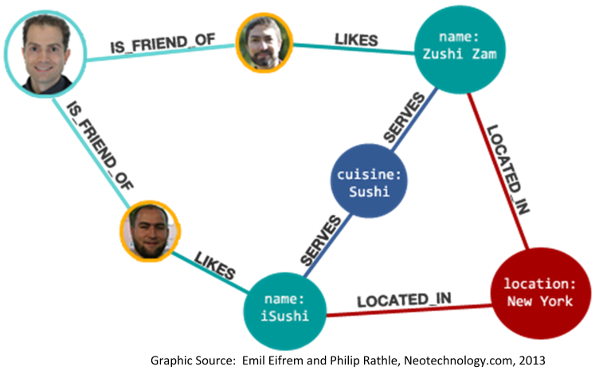
\includegraphics[width= 0.45 \textwidth]{graphDB.png}
\end{center}
\caption{Ejemplo de una DBOG.}
\label{fig2}
\end{figure}

Como se observa, el diagrama es bastante intuitivo de lo que nosotros entendemos por una relación. \\
Neo4j usa grafos de propiedad. Son grafos con peso, con etiquetas y donde podemos asignar propiedades tanto a nodos como relaciones (por
ejemplo, cuestiones como nombre, edad, país de residencia,nacimiento). 


\section{Instalación}
El proceso de instalación del programa Neo4j es diferente para cada sistema operativo. En el presente documento se explicará el proceso para la instalación en Windows y en una distribución de Linux (Ubuntu).\\
Se recomienda visitar la página de Neo4j para mayor información: 
\begin{itemize}
\item Requerimientos: https://neo4j.com/docs/operations-manual/current/installation/requirements/ 
\item Instalación para distribuciones Linux de Debian (Ubuntu):  https://neo4j.com/docs/operations-manual/current/installation/linux/debian/
\item Instalación para sistemas Window: https://neo4j.com/docs/operations-manual/current/installation/windows/
\end{itemize}

\subsection{Instalación en Windows}\label{AA}
Para instalar Neo4j en un computador (o servidor) con Windows se debe descargar el instalador de la página: https://neo4j.com/download/ \\
Una vez se haya descargado, se debe dar doble clic para ejecutarlo y se deben seguir las instrucciones. \\
Después de aceptar el acuerdo de licencia se mostrará la siguiente ventana, como se observa en la Figura \ref{fig3}.

\begin{figure}[H]
\begin{center}
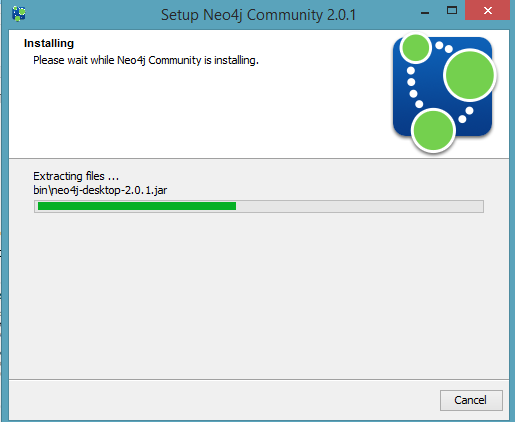
\includegraphics[width= 0.45 \textwidth]{neo4j_install02.png}
\end{center}
\caption{Instalación de Neo4j en Windows.}
\label{fig3}
\end{figure}

Una vez termine el proceso de instalación, se debe ejecutar Neo4j. Se abrirá la ventana que se muestra en la Figura \ref{fig4}.

\begin{figure}[H]
\begin{center}
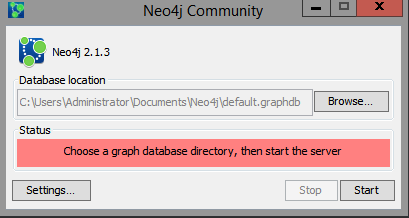
\includegraphics[width= 0.45 \textwidth]{neo4j_install06.png}
\end{center}
\caption{Ejecución de Neo4j en Windows.}
\label{fig4}
\end{figure}

Si se desea realizar configuraciones como
la cantidad de memoria RAM asignad a los nodos y las aristas, la configuración del acceso desde el explorador o desde un sitio remoto, el puerto de la conexión a la base de datos, habilitar auto indexación, entre otras opciones, se debe dar clic en Settings... Se desplegará una ventana como la que se muestra en la Figura \ref{fig5}.

\begin{figure}[H]
\begin{center}
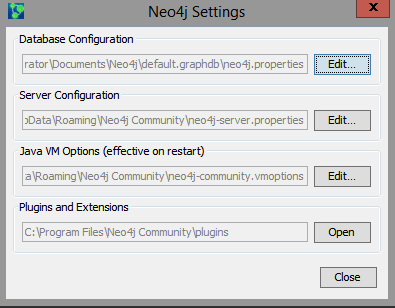
\includegraphics[width= 0.45 \textwidth]{neo4j_install07.png}
\end{center}
\caption{Configuraciones de Neo4j en Windows.}
\label{fig5}
\end{figure}

Finalmente, hechas las configuraciones deseadas, se debe dar clic en Start para hacer que el servidor arranque. La ventana de Neo4j debe quedar como en la Figura \ref{fig6}.

\begin{figure}[H]
\begin{center}
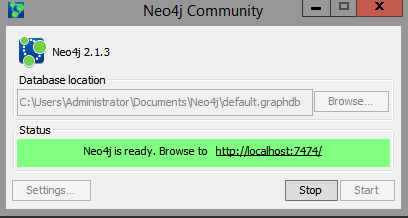
\includegraphics[width= 0.45 \textwidth]{neo4j_install09.png}
\end{center}
\caption{Arranque de Neo4j en Windows.}
\label{fig6}
\end{figure}

\subsection{Instalación en Linux (Debian/Ubuntu)}

Para las distribuciones de Linux el proceso es diferente. Es recomendable ir a la página https://neo4j.com/docs/operations-manual/current/installation/linux/debian/ para mayor información. \\
Para instalarlo se debe cumplir con el requisito de tener instalado Java 8 runtime. Para ello se debe ejecutar las siguientes sentencias, para tener acceso al repositorio e Java 8, como se muestran en las Figuras \ref{fig7} y \ref{fig8} 


\begin{figure}[H]
\begin{center}
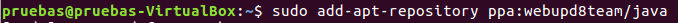
\includegraphics[width= 0.45 \textwidth]{java_repo.png}
\end{center}
\caption{Agregar repositorio de Java Runtime.}
\label{fig7}
\end{figure}

\begin{figure}[H]
\begin{center}
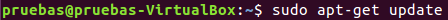
\includegraphics[width= 0.45 \textwidth]{sudo_update.png}
\end{center}
\caption{Actualizar repositorios de Linux.}
\label{fig8}
\end{figure}

Se usa la siguiente sentencia para poder instalar como tal el runtime de Java, como se observa en la Figura \ref{fig9}

\begin{figure}[H]
\begin{center}
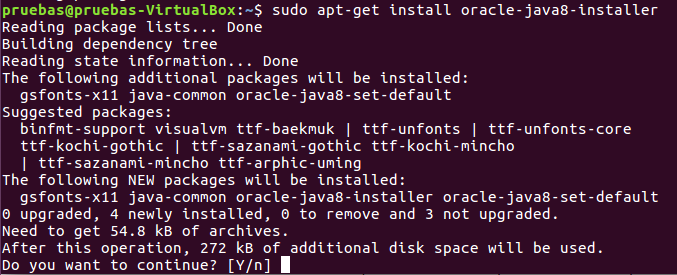
\includegraphics[width= 0.45 \textwidth]{install_java.png}
\end{center}
\caption{Instalación del Runtime de Java en Linux.}
\label{fig9}
\end{figure}

%sudo apt-get -t jessie-backports install ca-certificates-java

Una vez hecho esto, se debe agregar el repositorio de Neo4j. Para ello se ejecuta la siguiente sentencia desde la terminal, como se muestra en la Figura \ref{fig10}.

\begin{figure}[H]
\begin{center}
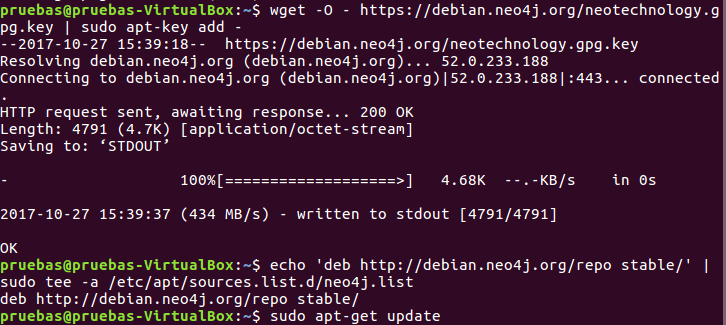
\includegraphics[width= 0.45 \textwidth]{neo4j_repo_f.png}
\end{center}
\caption{Repositorios de Neo4j en Linux.}
\label{fig10}
\end{figure}

Finalmente, se instala Neo4j, haciendo lo que se muestra en la Figura \ref{fig11}.

\begin{figure}[H]
\begin{center}
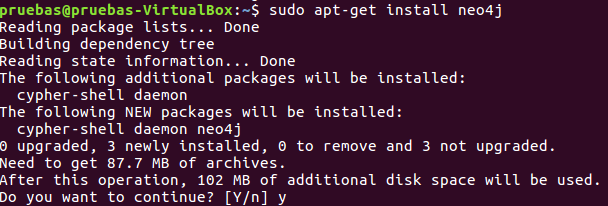
\includegraphics[width= 0.45 \textwidth]{install_neo4j.png}
\end{center}
\caption{Repositorios de Neo4j en Linux.}
\label{fig11}
\end{figure}

Para iniciar el servidor y arrancar en gestor de base de datos, se debe ejecutar el comando que se muestra en al Figura \ref{fig12}.

\begin{figure}[H]
\begin{center}
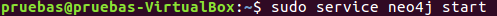
\includegraphics[width= 0.45 \textwidth]{start_service_neo.png}
\end{center}
\caption{Inicio del servidor de Neo4j en Linux.}
\label{fig12}
\end{figure}

\subsection{Prueba de la instalación}

Sin importar qué distribución  o qué sistema operativo se haya utilizado, se puede probar la correcta instalación utilizando el explorador Web. Se dirige a la dirección $localhost:7474/browser/$. 
\\
En esta dirección se tendrá todo el acceso y gestión de la base de datos: es un aplicativo corriendo sobre un explorador Web. Esto se muestra en la Figura \ref{fig13}.

\begin{figure}[H]
\begin{center}
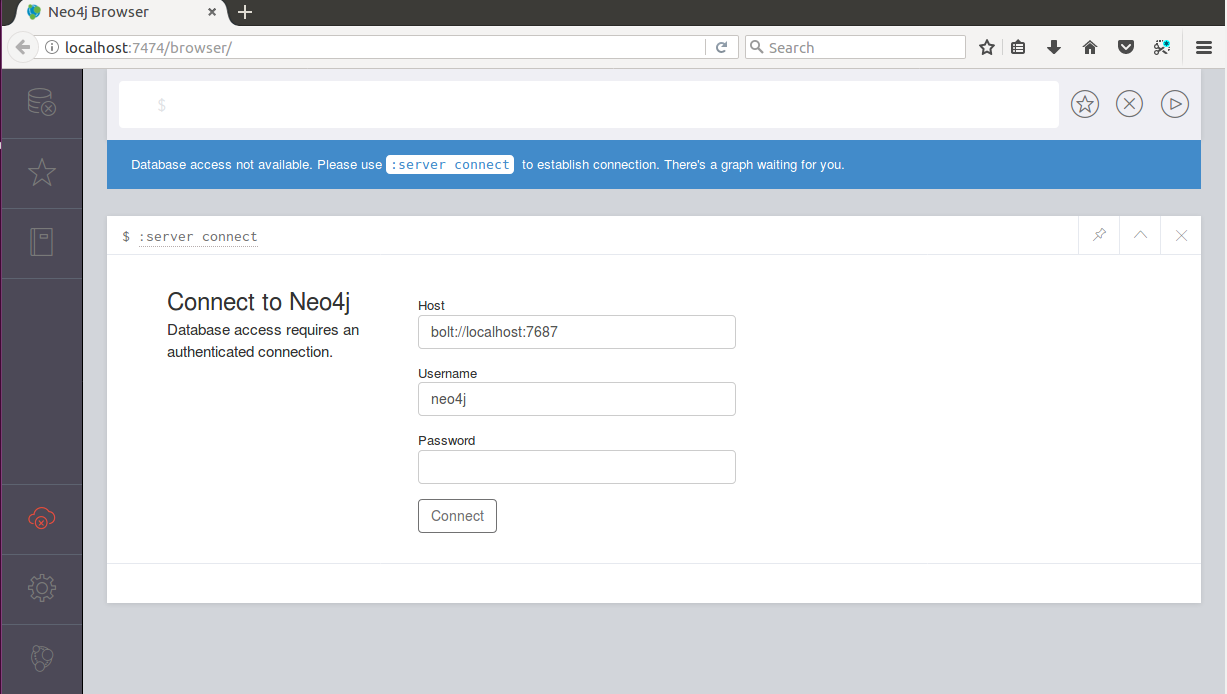
\includegraphics[width= 0.45 \textwidth]{web_browser1.png}
\end{center}
\caption{Neo4j corriendo desde el explorador Web.}
\label{fig13}
\end{figure}

La contraseña al iniciar Neo4j por primera vez por defecto es $neo4j$. Luego de ingresarla se pedirá se cambia la contraseña, como se muestra en la Figura \ref{fig14}.

\begin{figure}[H]
\begin{center}
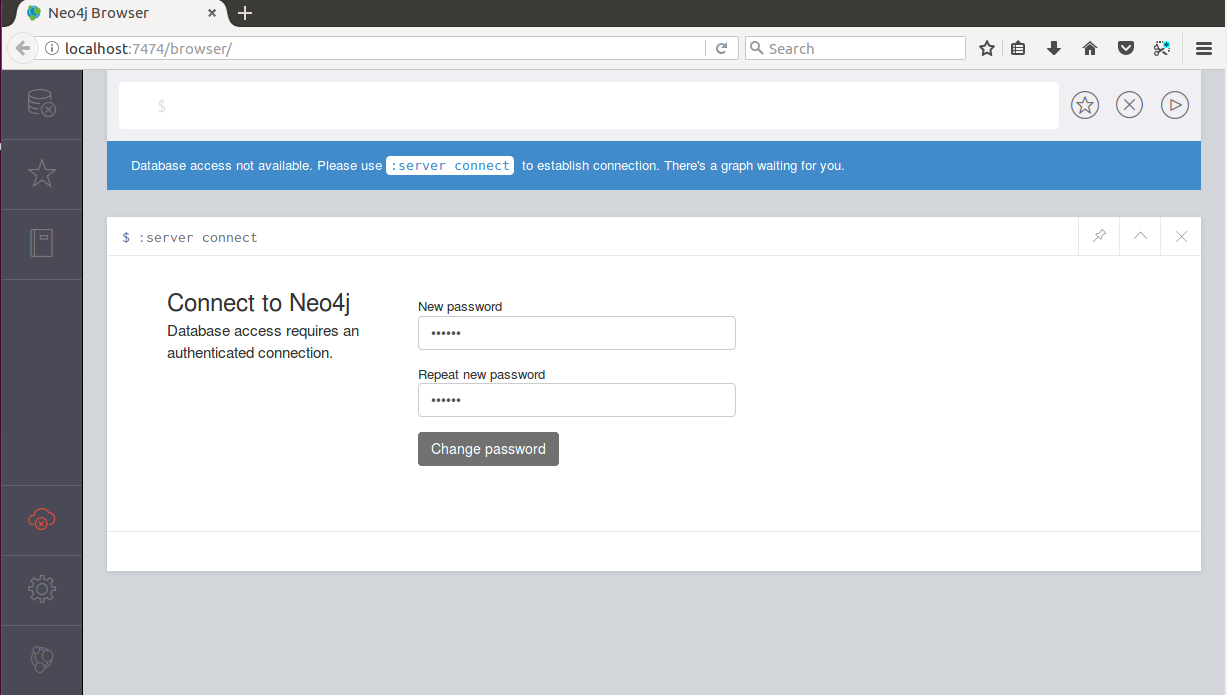
\includegraphics[width= 0.45 \textwidth]{web_change_p.png}
\end{center}
\caption{Cambio de contraseña en Neo4j por primera vez.}
\label{fig14}
\end{figure}

Una vez hecho esto, se estará en la página de inicio de Neo4j. Se verá la barra de ingreso de comandos (consultas), un espacio con las noticias y principales mensajes, un menú de accesos en el costado izquierdo y la conexión al servidor en sí. Todo esto se ilustra en la Figura \ref{fig15}.

\begin{figure}[H]
\begin{center}
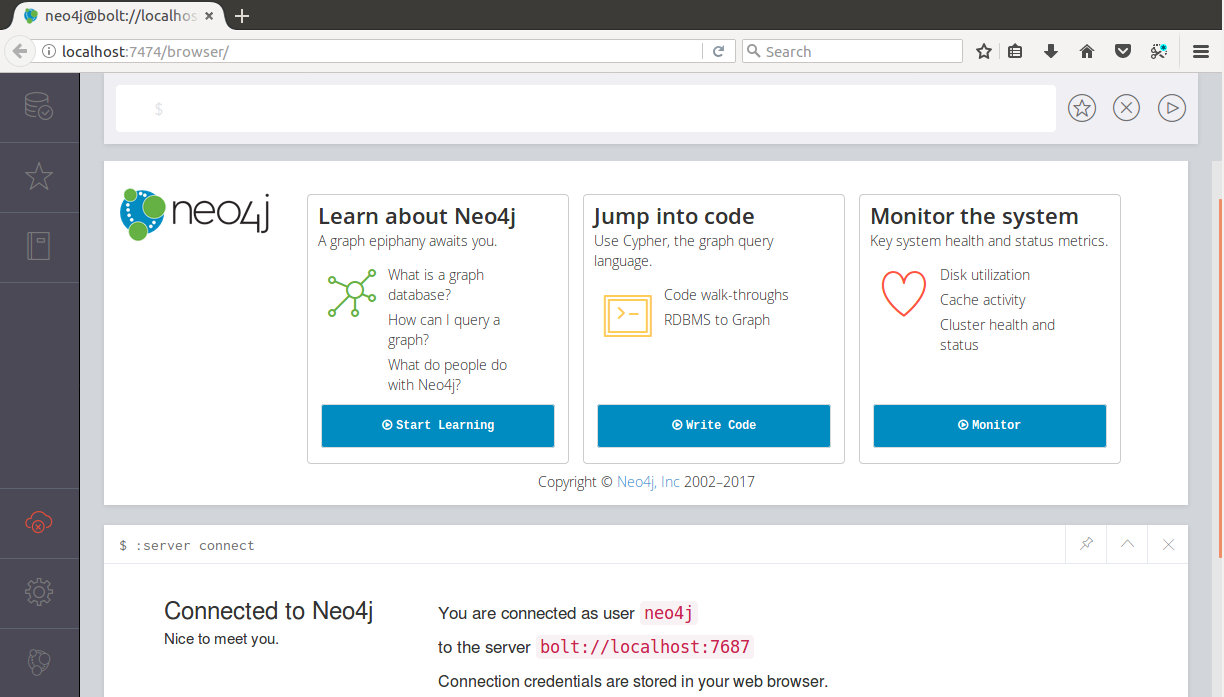
\includegraphics[width= 0.45 \textwidth]{inicio_neo4j.png}
\end{center}
\caption{Página de inicio de Neo4j.}
\label{fig15}
\end{figure}

\section{Creación de nodos.}

Una vez en el aplicativo de explorador se pueden crear nodos usando la sentencia \texttt{\textcolor{green}{CREATE} (\textcolor{blue}{n})}. Al ejecutar la sentencia se verá un mensaje que dice que se creó un nodo en un tiempo determinado. Si se desea observar el nodo, se debe crear de esta manera: \texttt{\textcolor{green}{CREATE} (\textcolor{blue}{n}) \textcolor{green}{RETURN} \textcolor{blue}{n}}. Esto se muestra en la Figura  \ref{fig16}.

\begin{figure}[H]
\begin{center}
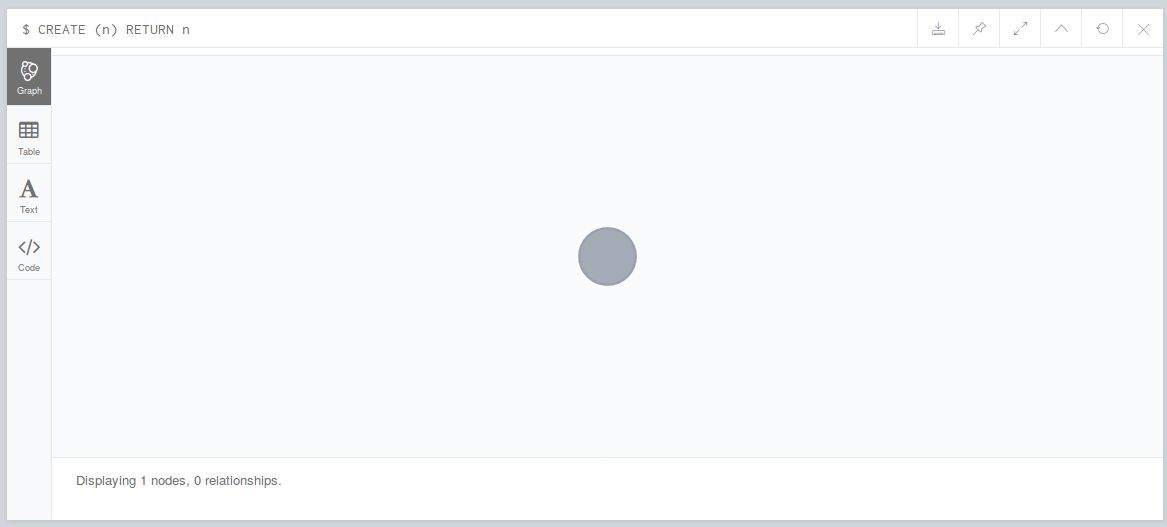
\includegraphics[width= 0.45 \textwidth]{create_node1.png}
\end{center}
\caption{Creación y visualización de un nodo.}
\label{fig16}
\end{figure}

Así mismo es posible crear varios nodos al tiempo y visualizarlos con el comando \texttt{\textcolor{green}{CREATE} (\textcolor{blue}{n}),(\textcolor{blue}{m}) \textcolor{green}{RETURN} \textcolor{blue}{n},\textcolor{blue}{m}}. 
\\
Un concepto importante en los nodos de Neo4j, son los label. Esta es una característica que define a qué grupo, clase o categoría pertenece el nodo. Por ejemplo, podemos crear nodos que pertenezcan y hagan referencia a personas. 
\\
Para agregar un label se hace de la siguiente manera: \texttt{\textcolor{green}{CREATE} (\textcolor{blue}{n}\textcolor{red}{:Persona}) \textcolor{green}{RETURN} \textcolor{blue}{n}}. Se debe aclarar aquí que la letra \texttt{n} es únicamente una referencia al nodo dentro de la sentencia específica. Bien se podría llamarlo o hacer referencia de otra manera y no cambiaría nada en el resultado. Por ejemplo \texttt{\textcolor{green}{CREATE} (\textcolor{blue}{yo}\textcolor{red}{:Persona}) \textcolor{green}{RETURN} \textcolor{blue}{yo}}. El resultado se muestra en la Figura \ref{fig17}.

\begin{figure}[H]
\begin{center}
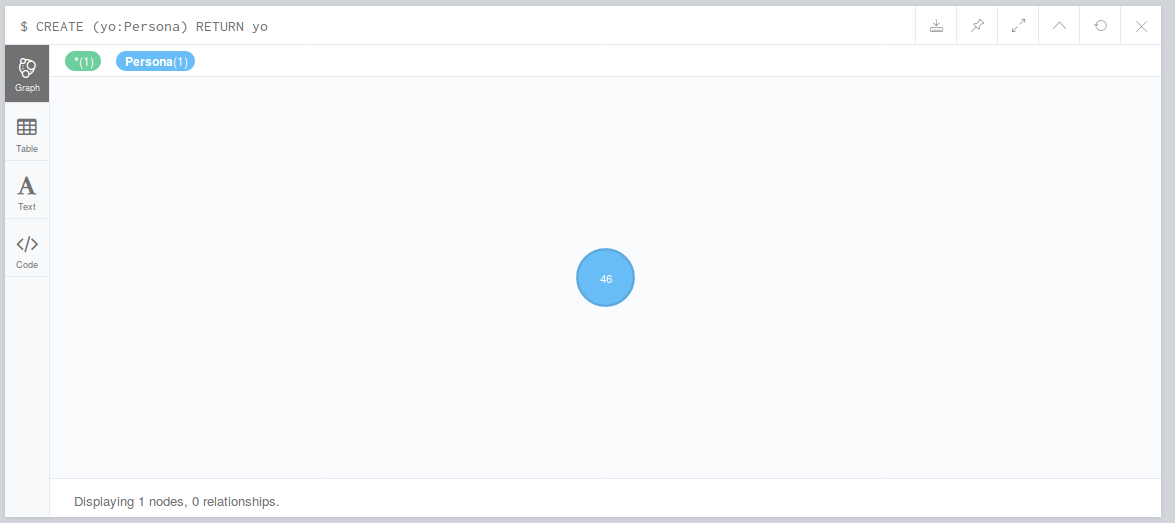
\includegraphics[width= 0.45 \textwidth]{crear_nodo_label1.png}
\end{center}
\caption{Nodo con label.}
\label{fig17}
\end{figure}

El número que se encuentra dentro del nodo (el círculo) es el id. Este es un identificador único de cada nodo. Si se posiciona el cursor sobre el nodo se observará que dice id.
\\
Dependiendo de la aplicación Neo4j permite tener más de un label para un nodo. Este sería el caso, por ejemplo, para nodos que pertenezcan a dos o más categorías. Un ejemplo sería una persona que tenga una nacionalidad. Esto se realiza agregando labels con : de manera consecutiva. Se puede usar la siguiente sentencia como ejemplo: \texttt{\textcolor{green}{CREATE} (\textcolor{blue}{persona}\textcolor{red}{:Persona:Colombia}) \textcolor{green}{RETURN} \textcolor{blue}{persona}}. Esto se observa en la Figura \ref{fig18}.

\begin{figure}[H]
\begin{center}
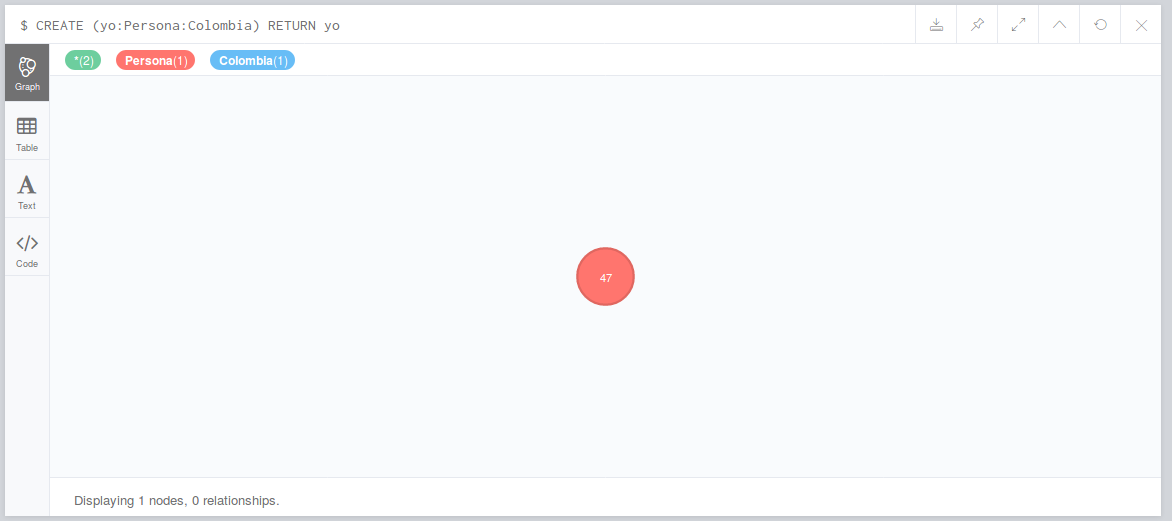
\includegraphics[width= 0.45 \textwidth]{crear_nodo_label2.png}
\end{center}
\caption{Nodo con dos label.}
\label{fig18}
\end{figure}

Hasta este punto se han creado nodos que pertenecen a una o más categorías. Ahora hace falta añadir información a cada nodo. Esto se realiza por medio de las propiedades. Para agregar información se escribe dentro de \{ \} al momento de crear el nodo (se puede agregar o editar información luego de crearlos). La información se agrega escribiendo el nombre del campo seguido de : y finalmente el valor. El valor puede ser numérico (entero o de coma flotante), un string, valor booleano o un arregla del mismo tipo de datos.
\\
Un ejemplo de la creación de un nodo con propiedades es usando la siguiente sentencia:  \texttt{\textcolor{green}{CREATE} (\textcolor{blue}{persona}\textcolor{red}{:Persona} \{ name:  "\textcolor{brown}{Mi nombre}" \} ) \textcolor{green}{RETURN} \textcolor{blue}{persona}}. Así mismo se pueden agregar más propiedades. Esto se muestra en la Figura \ref{fig19}.

\begin{figure}[H]
\begin{center}
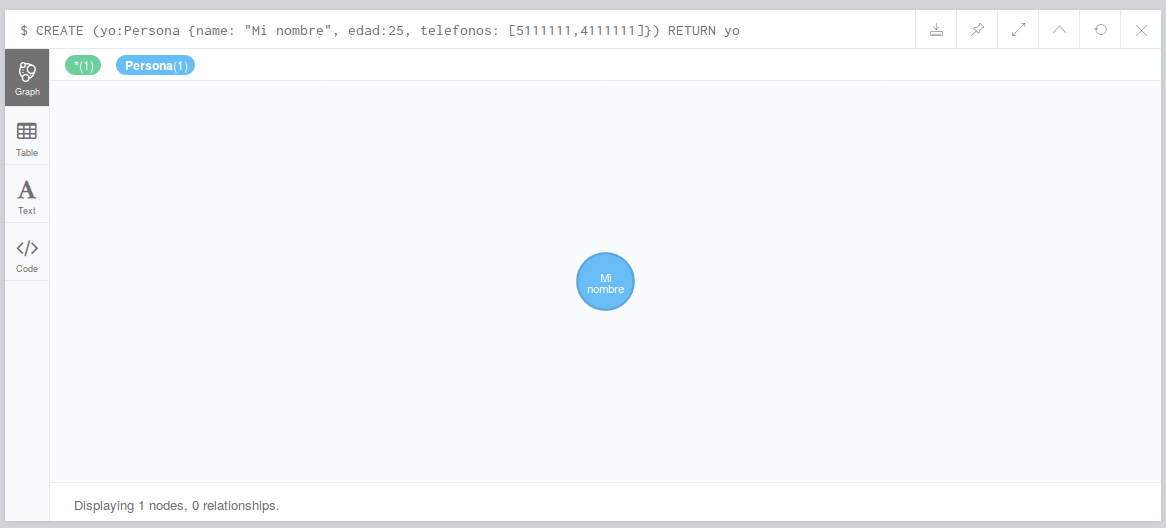
\includegraphics[width= 0.45 \textwidth]{crear_nodo_prop1.png}
\end{center}
\caption{Nodo con propiedades.}
\label{fig19}
\end{figure}


\section{Consultas básicas.}

Para hacer consultas en Neo4j se utiliza la palabra clave \texttt{\textcolor{green}{MATCH}}. Esta palabra va seguido de la información del nodo o nodos que se desean consultar. Por ejemplo, si se busca por algún label específico, por el valor de alguna propiedad o hasta por una relación (se verá en la siguiente sección). Luego, algo importante, es utilizar la sentencia \texttt{\textcolor{green}{RETURN}}, con el fin de ver los nodos encontrados. Un ejemplo clásico que retorna todos los nodos existentes es la siguiente sentencia \texttt{\textcolor{green}{MATCH} (\textcolor{blue}{n}) \textcolor{green}{RETURN} \textcolor{blue}{n}}. El resultado se observa en la Figura \ref{fig20}.


\begin{figure}[H]
\begin{center}
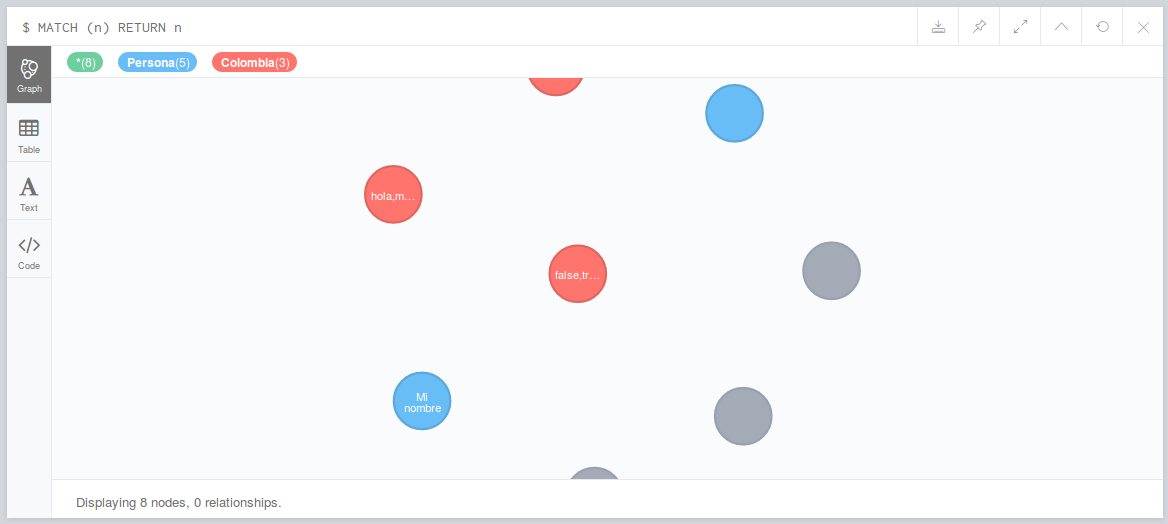
\includegraphics[width= 0.45 \textwidth]{consulta_todo1.png}
\end{center}
\caption{Consulta de todos los nodos.}
\label{fig20}
\end{figure}

Como se observa, si se tuviera una base de datos extensa, se tendría problemas para visualizar los nodos. Es por esto que es recomendable limitar el número de resultados. Para hacer esto se utiliza la sentencia \texttt{\textcolor{green}{LIMIT}} seguida del número de nodos máximos que se desea aparezcan. Por ejemplo, se usaría la sentencia \texttt{\textcolor{green}{MATCH} (\textcolor{blue}{n}) \textcolor{green}{RETURN} \textcolor{blue}{n} \textcolor{green}{LIMIT} \textcolor{blue}{4}}. El resultado se observa en la Figura \ref{fig21}.

\begin{figure}[H]
\begin{center}
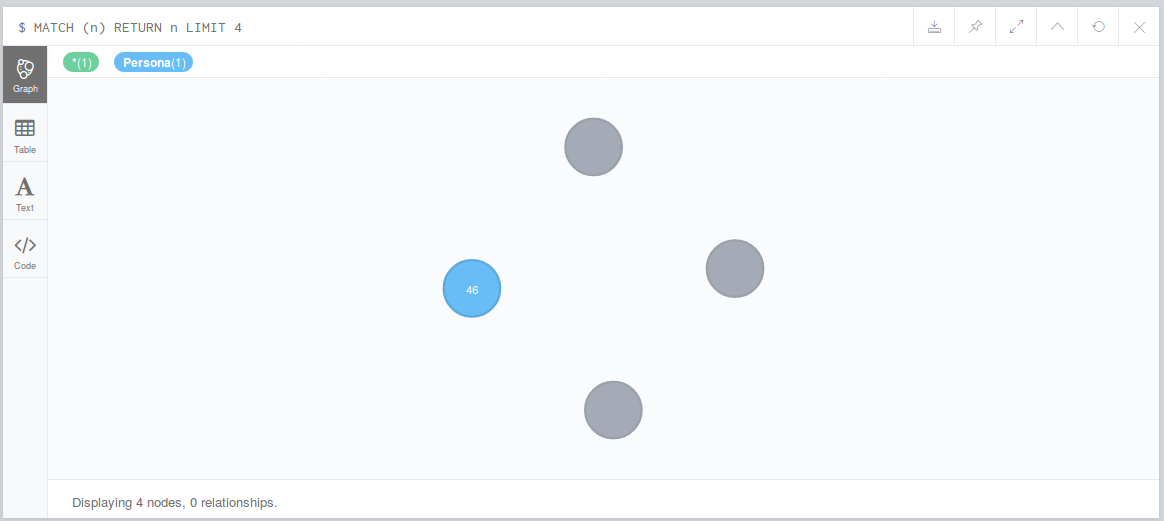
\includegraphics[width= 0.45 \textwidth]{consulta_limite1.png}
\end{center}
\caption{Consulta de los nodos con límite de 4.}
\label{fig21}
\end{figure}

Si se quiere buscar los nodos que pertenezcan a la misma categoría, grupo, clase o label, se debe especificar el label. Para ello se hace lo mismo que cuando se crea un nodo de una categoría. Es decir, se utiliza la sentencia \texttt{(\textcolor{blue}{n}\textcolor{red}{:Label})} en vez de \texttt{(\textcolor{blue}{n})}. Por ejemplo, al buscar todos los nodos que pertenezcan a personas se utilizaría la sentencia \texttt{\textcolor{green}{MATCH} (\textcolor{blue}{n}\textcolor{red}{:Persona}) \textcolor{green}{RETURN} \textcolor{blue}{n} \textcolor{green}{LIMIT} \textcolor{blue}{4}}. El resultado se observa en la Figura \ref{fig22}.


\begin{figure}[H]
\begin{center}
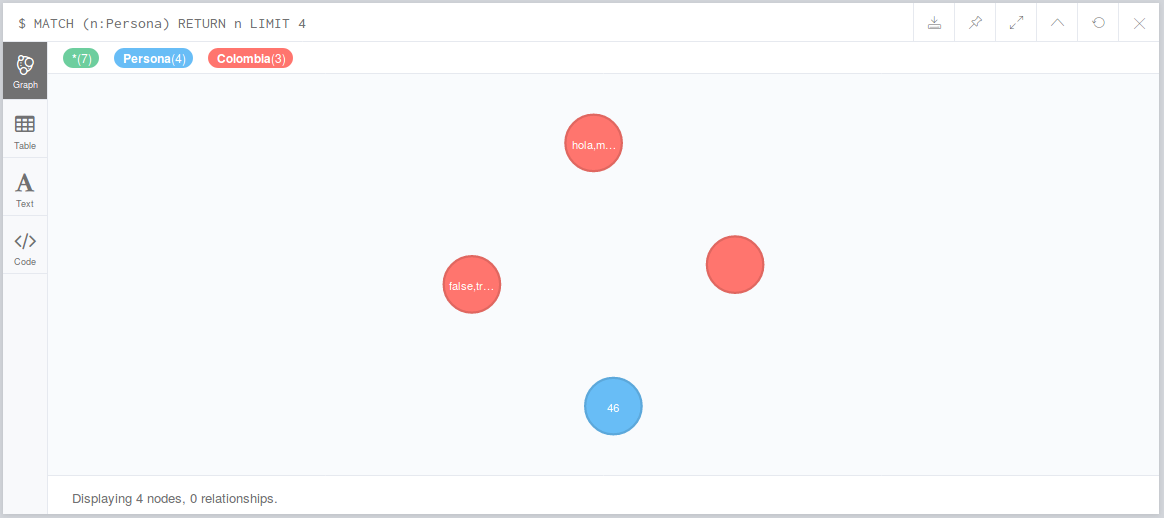
\includegraphics[width= 0.45 \textwidth]{consulta_label1.png}
\end{center}
\caption{Consulta de los nodos que pertenezcan a Persona.}
\label{fig22}
\end{figure}

Otra manera de consultar nodos y filtrarlos es por sus propiedades. Se podría preguntar por los nodos que tengan cierto nombre. La sentencia es similar a la manera que se creó un nodo con propiedades, usando \{ \} e ingresando las propiedades dentro. Por ejemplo, se podría buscar los nodos que tengan el nombre "Mi nombre". Para ello se utiliza al sentencia \texttt{\textcolor{green}{MATCH} (\textcolor{blue}{n} \{ name: "\textcolor{brown}{Mi nombre}" \}) \textcolor{green}{RETURN} \textcolor{blue}{n} \textcolor{green}{LIMIT} \textcolor{blue}{4}}. Se insiste que la letra \texttt{\textcolor{blue}{n}} es el nombre que se le asigna a los nodos encontrados en esta sentencia. De manera que bien se podría utilizar otra letra o cualquier palabra, sin cambiar el resultado. También es posible hacer la consulta buscando por los nodos que tengan el nombre "Mi nombre" y que además perezcan a Personas. Esto se muestra en la siguiente sentencia \texttt{\textcolor{green}{MATCH} (\textcolor{blue}{yo}\textcolor{red}{:Persona} \{ name: "\textcolor{brown}{Mi nombre}" \}) \textcolor{green}{RETURN} \textcolor{blue}{yo} \textcolor{green}{LIMIT} \textcolor{blue}{4}}. El resultado se observa en la Figura \ref{fig23}

\begin{figure}[H]
\begin{center}
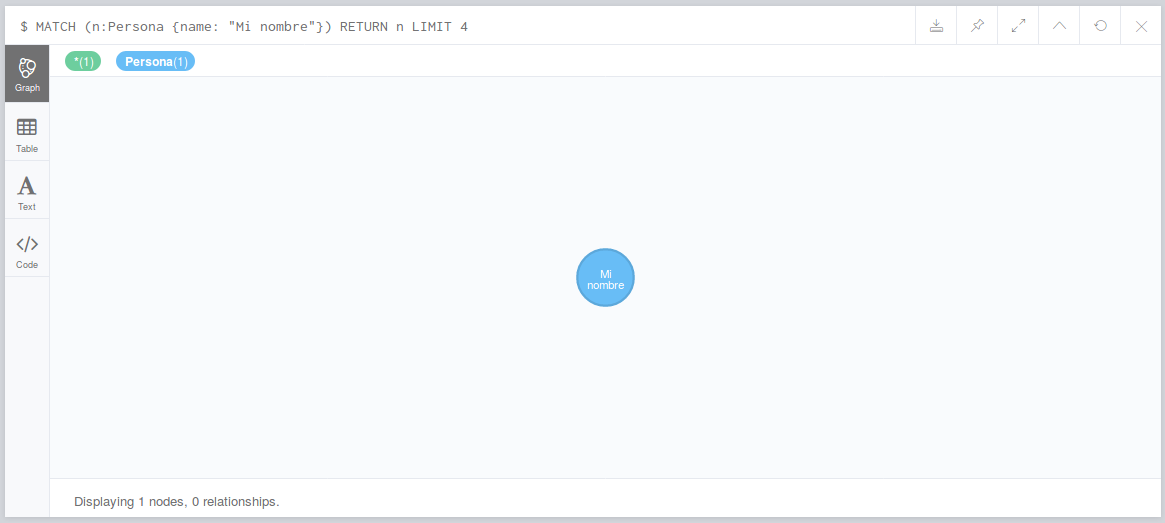
\includegraphics[width= 0.45 \textwidth]{consulta_label2.png}
\end{center}
\caption{Consulta de los nodos que pertenezcan a Persona y se llaman "Mi nombre".}
\label{fig23}
\end{figure}

Para finalizar con las consultas básicas se va a utilizar un último criterio de búsqueda: consultas por el id del nodo. Para conocer todas las propiedades de un nodo, se debe posicionar el cursor sobre el nodo deseado y aparecerán las propiedades en la parte inferior. Junto a las propiedades se observa el id del nodo dentro de $<$ $>$. Esto se observa en la Figura \ref{fig24}.

\begin{figure}[H]
\begin{center}
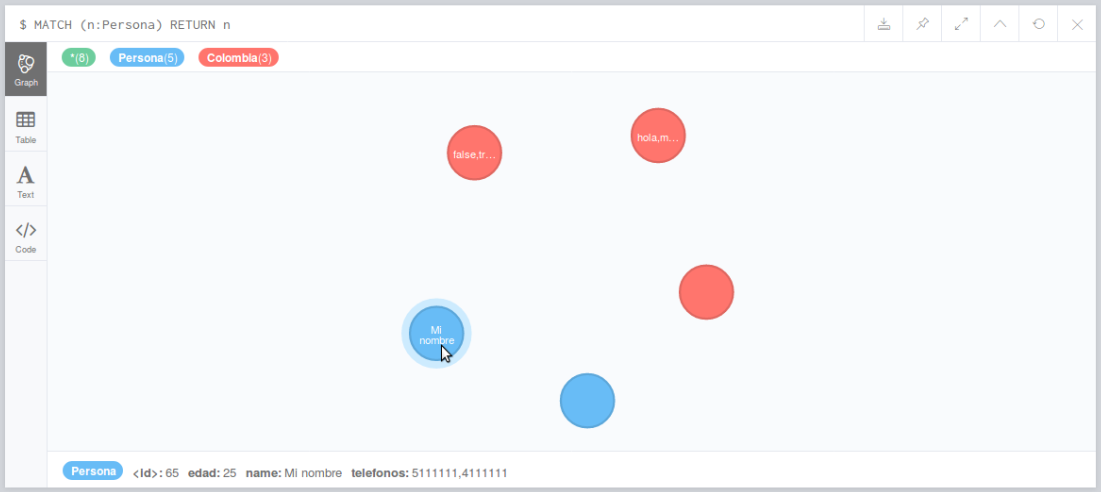
\includegraphics[width= 0.45 \textwidth]{nodo_id.png}
\end{center}
\caption{Visualización de las propiedades del nodo.}
\label{fig24}
\end{figure}

Para consultar por el id del nodo se utiliza simplemente la condición \texttt{\textcolor{green}{WHERE} \textcolor{blue}{id}(\textcolor{blue}{n})=\textcolor{blue}{65}}. El número 65 es un ejemplo para este caso. La consulta completa quedaría así \texttt{\textcolor{green}{MATCH} (\textcolor{blue}{n}) \textcolor{green}{WHERE} \textcolor{blue}{id}(\textcolor{blue}{n})=\textcolor{blue}{65} \textcolor{green}{RETURN} \textcolor{blue}{n}}. El resultado se observa en la Figura \ref{fig25}.

\begin{figure}[H]
\begin{center}
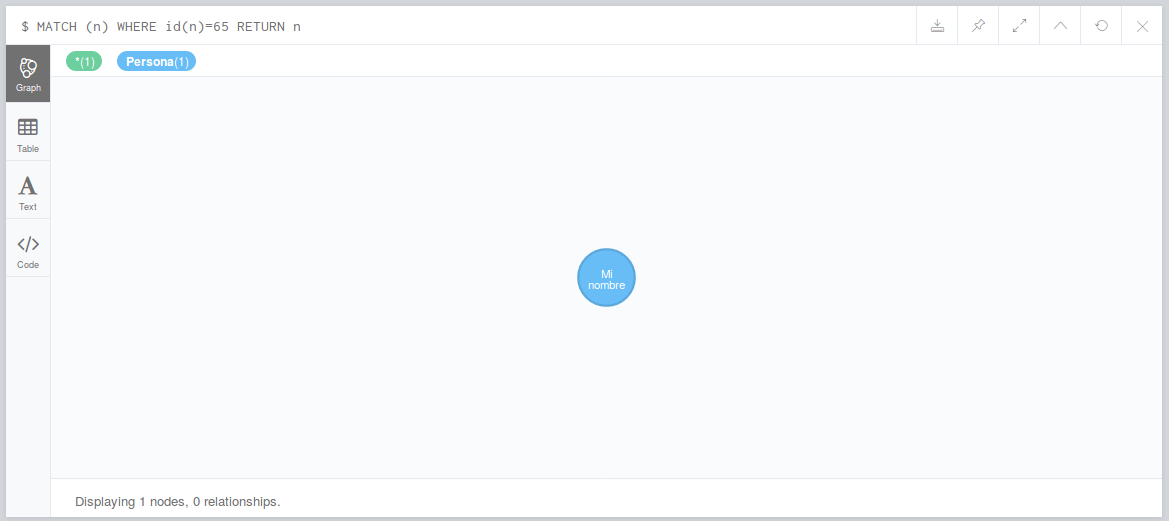
\includegraphics[width= 0.45 \textwidth]{consulta_id.png}
\end{center}
\caption{Consulta del nodo por el id.}
\label{fig25}
\end{figure}

\section{Cambiar o agregar propiedades de los nodos.}

Para cambiar o añadir alguna propiedad a un nodo ya creado, se debe primero realizar una consulta que direccione hacia dicho nodo. Por ejemplo, de los nodos creados el nodo con id 43 no pertenece a ninguna categoría, ningún label. Primero se debe asegurar es el nodo deseado, así que se ejecuta la consulta \texttt{\textcolor{green}{MATCH} (\textcolor{blue}{n}) \textcolor{green}{WHERE} \textcolor{blue}{id}(\textcolor{blue}{n})=\textcolor{blue}{43} \textcolor{green}{RETURN} \textcolor{blue}{n}}. El resultado de la consulta se observa en la Figura \ref{fig26}.

\begin{figure}[H]
\begin{center}
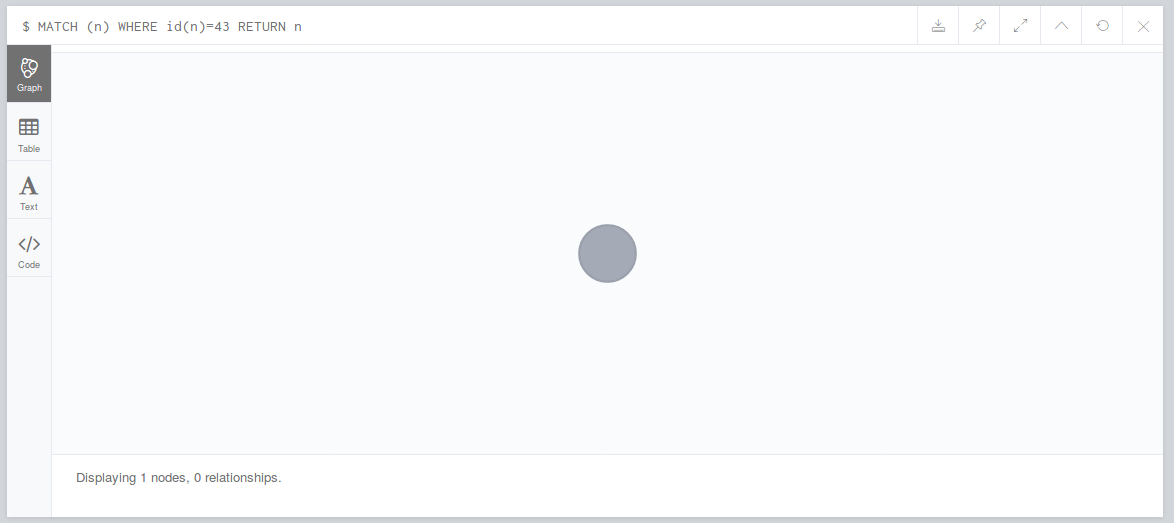
\includegraphics[width= 0.45 \textwidth]{consulta_id2.png}
\end{center}
\caption{Consulta del nodo por el id.}
\label{fig26}
\end{figure}

Ahora, se utiliza la palabra reservada \texttt{\textcolor{green}{SET}} para cambiar alguna propiedad o algún Label. En este caso se quiere cambiar el label, así que se utiliza la consulta seguida de la sentencia \texttt{\textcolor{green}{SET} \textcolor{blue}{n}\textcolor{red}{:Persona}}. La sentencia quedaría así: \texttt{\textcolor{green}{MATCH} (\textcolor{blue}{n}) \textcolor{green}{WHERE} \textcolor{blue}{id}(\textcolor{blue}{n})=\textcolor{blue}{43} \textcolor{green}{SET} \textcolor{blue}{n}\textcolor{red}{:Persona} \textcolor{green}{RETURN} \textcolor{blue}{n}}. El resultado se observa en la Figura \ref{fig27}.


\begin{figure}[H]
\begin{center}
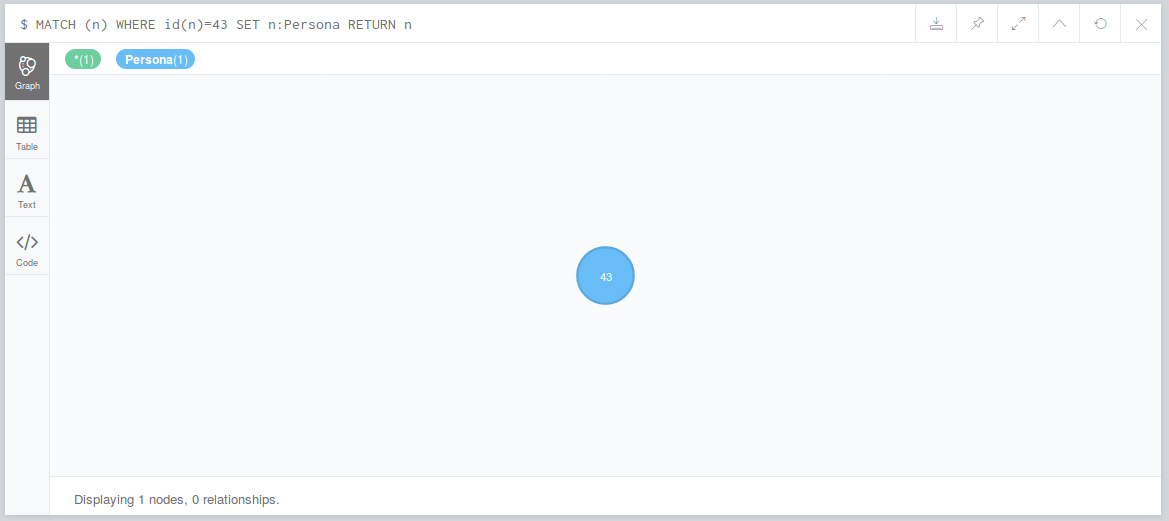
\includegraphics[width= 0.45 \textwidth]{set_label1.png}
\end{center}
\caption{Cambio del label de un nodo.}
\label{fig27}
\end{figure}

Si el nodo ya tenía un label, al hacer esta sentencia simplemente se agregaría un nuevo label. Para agregar dos o más labels en una sola sentencia se utiliza la misma lógica, solo que se agregan los labels deseados separados por : Esto se muestra en esta sentencia \texttt{\textcolor{green}{MATCH} (\textcolor{blue}{n}) \textcolor{green}{WHERE} \textcolor{blue}{id}(\textcolor{blue}{n})=\textcolor{blue}{43} \textcolor{green}{SET} \textcolor{blue}{n}\textcolor{red}{:Persona:Colombia} \textcolor{green}{RETURN} \textcolor{blue}{n}}
\\
Para agregar una propiedad o para cambiar el valor de una propiedad ya existente se utiliza la sentencia \texttt{\textcolor{green}{SET}} seguida del nombre que se desea asignar al nodo (normalmente \texttt{\textcolor{blue}{n}}) luego un punto ., seguido del nombre de la propiedad, luego el signo igual y finalmente el valor que deseamos asignar. Un ejemplo sería \texttt{\textcolor{green}{SET} \textcolor{blue}{n}.name= "\textcolor{brown}{Otro nombre}"}. En este caso, si la propiedad ya existe y tiene valor en dicho nodo, Neo4j cambiará el valor por el que se le está ingresando. En caso que no exista, se creará la propiedad y se asignará el valor. 
\\
Un ejemplo de agregar una propiedad sería el siguiente \texttt{\textcolor{green}{MATCH} (\textcolor{blue}{n}) \textcolor{green}{WHERE} \textcolor{blue}{id}(\textcolor{blue}{n})=\textcolor{blue}{64} \textcolor{green}{SET} \textcolor{blue}{n}.name= "\textcolor{brown}{Otro nombre}"  \textcolor{green}{RETURN} \textcolor{blue}{n}}. El resultado se muestra en la Figura \ref{fig28}.


\begin{figure}[H]
\begin{center}
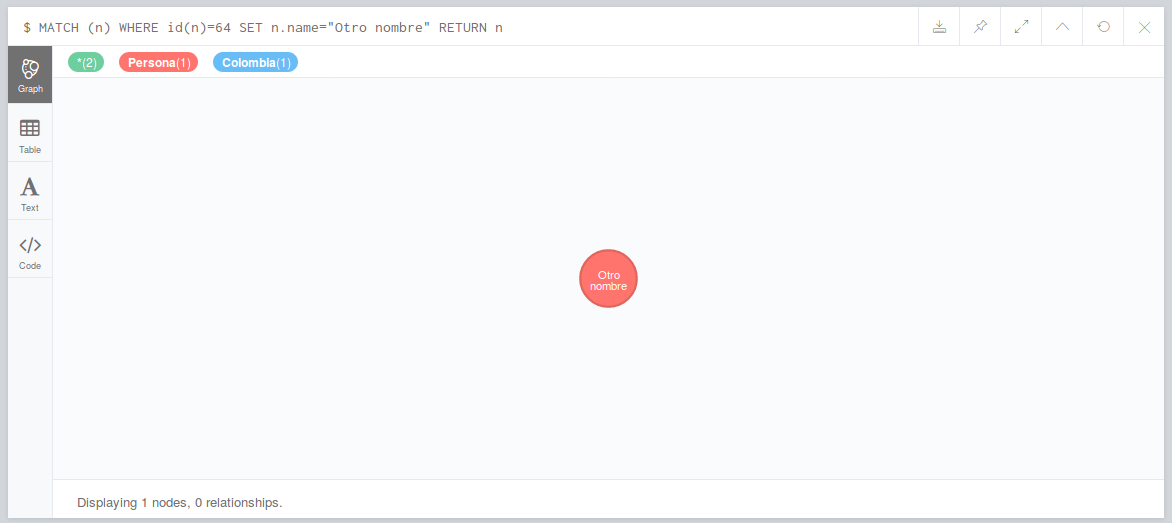
\includegraphics[width= 0.45 \textwidth]{set_nombre1.png}
\end{center}
\caption{Agregar la propiedad nombre de un nodo.}
\label{fig28}
\end{figure}

Otra manera de agregar o cambiar propiedades es utilizando una sentencia similar a la usada cuando se crearon las propiedades con los \{ \}. Aquí se debe tener cuidado. La sentencia \texttt{\textcolor{green}{SET}} quedaría así \texttt{\textcolor{green}{SET} \textcolor{blue}{n} += \{ name: "\textcolor{brown}{Otro nombre}" \}}. En este caso la sentencia buscaría si existe alguna propiedad \texttt{name}. Si es así cambia su valor a \texttt{"Otro nombre"}, sino la crea y asigna el valor. Si no se escribe el signo \texttt{+} junto al signo \texttt{=} se dejará como única propiedad la que se está asignando, es decir, se borrarán todas las demás propiedades. 
\\
Un ejemplo de agregar o editar una propiedad con este tipo de sentencias es el siguiente: \texttt{\textcolor{green}{MATCH} (\textcolor{blue}{n}) \textcolor{green}{WHERE} \textcolor{blue}{id}(\textcolor{blue}{n})=\textcolor{blue}{64} \textcolor{green}{SET} \textcolor{blue}{n} += \{ name: "\textcolor{brown}{Segundo nombre}" \}  \textcolor{green}{RETURN} \textcolor{blue}{n}}. El resutlado se muestra en la Figura \ref{fig29}.

\begin{figure}[H]
\begin{center}
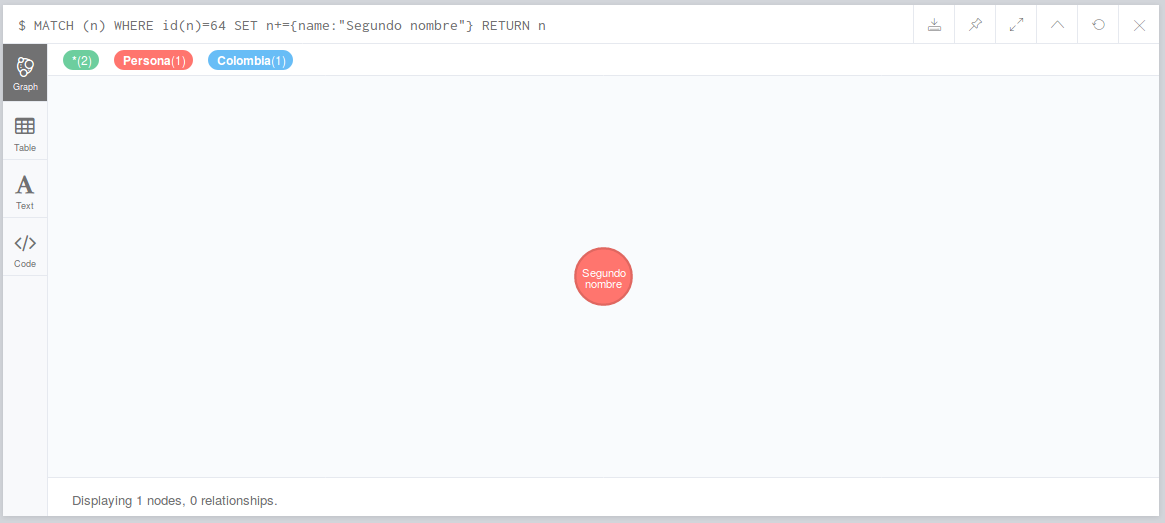
\includegraphics[width= 0.45 \textwidth]{set_nombre2.png}
\end{center}
\caption{Cambiar la propiedad nombre de un nodo.}
\label{fig29}
\end{figure}

Para eliminar una propiedad se realiza similar a establecer su valor. Solo que se asigna un valor nulo o \texttt{\textcolor{green}{null}}. Esta es una manera sencilla de hacerlo. Un ejemplo de esto se muestra en la sentencia \texttt{\textcolor{green}{MATCH} (\textcolor{blue}{n}) \textcolor{green}{WHERE} \textcolor{blue}{id}(\textcolor{blue}{n})=\textcolor{blue}{64} \textcolor{green}{SET} \textcolor{blue}{n}.name= \textcolor{green}{null}  \textcolor{green}{RETURN} \textcolor{blue}{n}}. El resultado se muestra en la Figura \ref{fig30}.

\begin{figure}[H]
\begin{center}
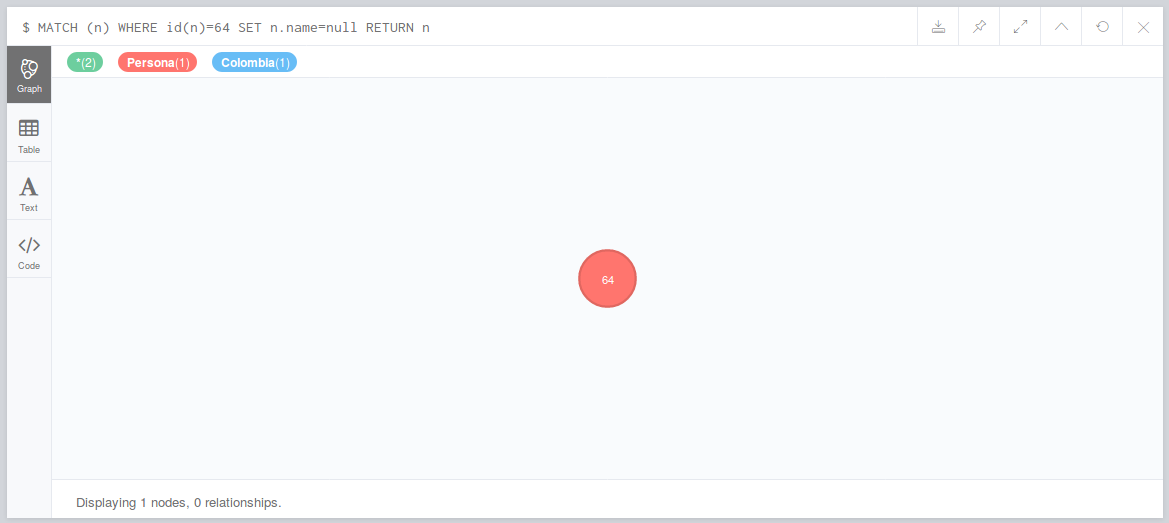
\includegraphics[width= 0.45 \textwidth]{set_nombre3.png}
\end{center}
\caption{Borrar la propiedad nombre de un nodo.}
\label{fig30}
\end{figure}

Otra manera se borrar una propiedad es utilizando la palabra clave \texttt{\textcolor{green}{REMOVE}}. Se usa de manera similar a la palabra \texttt{\textcolor{green}{SET}}, pero no se asigna valor a la propiedad. Por ejemplo se usaría simplemente \texttt{\textcolor{green}{REMOVE} \textcolor{blue}{n}.name}. Una sentencia de ejemplo sería \texttt{\textcolor{green}{MATCH} (\textcolor{blue}{n}) \textcolor{green}{WHERE} \textcolor{blue}{id}(\textcolor{blue}{n})=\textcolor{blue}{64} \textcolor{green}{REMOVE} \textcolor{blue}{n}.name  \textcolor{green}{RETURN} \textcolor{blue}{n}}. El resultado se muestra en la Figura \ref{fig31}.

\begin{figure}[H]
\begin{center}
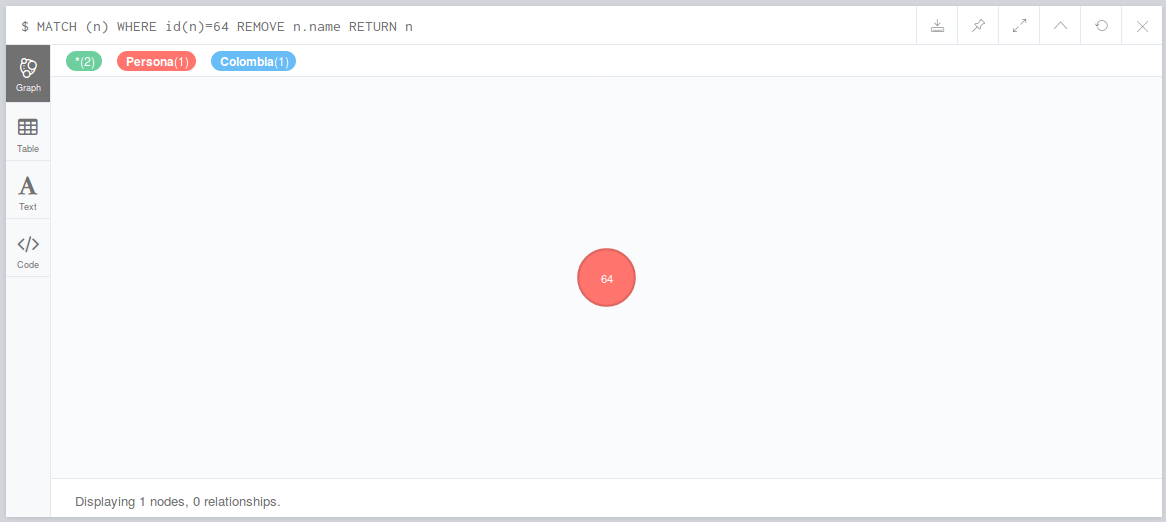
\includegraphics[width= 0.45 \textwidth]{remove_nombre1.png}
\end{center}
\caption{Borrado de la propiedad nombre de un nodo.}
\label{fig31}
\end{figure}

Finalmente con la misma sentencia \texttt{\textcolor{green}{REMOVE}} se puede borrar labels se un nodo. Se hace de la misma manera que se asignaron con la sentencia \texttt{\textcolor{green}{SET}}. Un ejemplo sería el siguiente \texttt{\textcolor{green}{REMOVE} \textcolor{blue}{n}\textcolor{red}{:Colombia}}. La sentencia quedaría así: \texttt{\textcolor{green}{MATCH} (\textcolor{blue}{n}) \textcolor{green}{WHERE} \textcolor{blue}{id}(\textcolor{blue}{n})=\textcolor{blue}{43} \textcolor{green}{REMOVE} \textcolor{blue}{n}\textcolor{red}{:Colombia} \textcolor{green}{RETURN} \textcolor{blue}{n}}. El resultado se observa en la Figura \ref{fig32}.

\begin{figure}[H]
\begin{center}
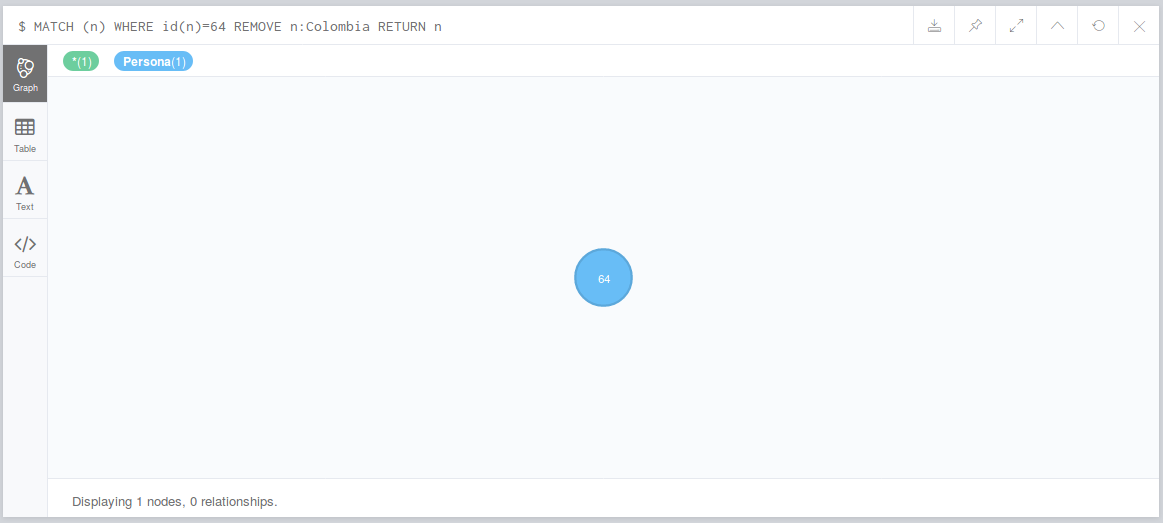
\includegraphics[width= 0.45 \textwidth]{remove_label1.png}
\end{center}
\caption{Borrado del label de un nodo.}
\label{fig32}
\end{figure}

\section{Creación de relaciones.}



\section*{Acknowledgment}

The preferred spelling of the word ``acknowledgment'' in America is without 
an ``e'' after the ``g''. Avoid the stilted expression ``one of us (R. B. 
G.) thanks $\ldots$''. Instead, try ``R. B. G. thanks$\ldots$''. Put sponsor 
acknowledgments in the unnumbered footnote on the first page.

\section*{References}

Please number citations consecutively within brackets \cite{b1}. The 
sentence punctuation follows the bracket \cite{b2}. Refer simply to the reference 
number, as in \cite{b3}---do not use ``Ref. \cite{b3}'' or ``reference \cite{b3}'' except at 
the beginning of a sentence: ``Reference \cite{b3} was the first $\ldots$''

Number footnotes separately in superscripts. Place the actual footnote at 
the bottom of the column in which it was cited. Do not put footnotes in the 
abstract or reference list. Use letters for table footnotes.

Unless there are six authors or more give all authors' names; do not use 
``et al.''. Papers that have not been published, even if they have been 
submitted for publication, should be cited as ``unpublished'' \cite{b4}. Papers 
that have been accepted for publication should be cited as ``in press'' \cite{b5}. 
Capitalize only the first word in a paper title, except for proper nouns and 
element symbols.

For papers published in translation journals, please give the English 
citation first, followed by the original foreign-language citation \cite{b6}.


\begin{thebibliography}{00}
\bibitem{b1} G. Eason, B. Noble, and I. N. Sneddon, ``On certain integrals of Lipschitz-Hankel type involving products of Bessel functions,'' Phil. Trans. Roy. Soc. London, vol. A247, pp. 529--551, April 1955.
\bibitem{b2} J. Clerk Maxwell, A Treatise on Electricity and Magnetism, 3rd ed., vol. 2. Oxford: Clarendon, 1892, pp.68--73.
\bibitem{b3} I. S. Jacobs and C. P. Bean, ``Fine particles, thin films and exchange anisotropy,'' in Magnetism, vol. III, G. T. Rado and H. Suhl, Eds. New York: Academic, 1963, pp. 271--350.
\bibitem{b4} K. Elissa, ``Title of paper if known,'' unpublished.
\bibitem{b5} R. Nicole, ``Title of paper with only first word capitalized,'' J. Name Stand. Abbrev., in press.
\bibitem{b6} Y. Yorozu, M. Hirano, K. Oka, and Y. Tagawa, ``Electron spectroscopy studies on magneto-optical media and plastic substrate interface,'' IEEE Transl. J. Magn. Japan, vol. 2, pp. 740--741, August 1987 [Digests 9th Annual Conf. Magnetics Japan, p. 301, 1982].
\bibitem{b7} M. Young, The Technical Writer's Handbook. Mill Valley, CA: University Science, 1989.
\end{thebibliography}


\end{document}
